% Uncomment this line for on-screen presentation
\documentclass[xcolor={dvipsnames}]{beamer}\usepackage{etoolbox}\newtoggle{printable}\togglefalse{printable}

% Uncomment this line for printable slides (disable animations and don't waste ink)
%\documentclass[handout, xcolor={dvipsnames}]{beamer}\usepackage{etoolbox}\newtoggle{printable}\toggletrue{printable}

% Adjust these for the path of the theme and its graphics, relative to this file
%\usepackage{beamerthemeFalmouthGamesAcademy}
\usepackage{../../beamerthemeFalmouthGamesAcademy}
\graphicspath{ {../../} }

% Default language for code listings
\lstset{language=C++,
		morekeywords={each,in}
}

\begin{document}
\title{Programming Practice II}   
\subtitle{BSc Computing for Games}

\frame{\titlepage} 

\part{Morning}
\frame{\partpage}

\begin{frame}{Game Design}
	In the morning session you will:
	
	\begin{itemize}
		\item Work individually.
		\item \textbf{Design} a simple 2D game.
		\begin{itemize}
			\item \textbf{Draw ONE} target audience card. 
			\item \textbf{Draw TWO} creativity cards. 
		\end{itemize}
		\item \textbf{Identify} the core-mechanic in the design \textbf{and create}
		a paper prototype of that mechanic.
	\end{itemize}
\end{frame}

\begin{frame}{Game Design}
	\begin{itemize}
		\item Reflect upon Friday’s COMP150 lecture content, focusing on the different forms of prototype which can be included in a pitch
		\item Use today’s practice session as an opportunity to develop the design you wish to pitch
		\item Review appropriate resources to help you with your activity:
		\begin{itemize}
			\item \url{http://video.mit.edu/watch/paper-prototyping-your-game-episode-1-part-1-5514/}
			\item \url{http://host.conseiljedi.com/~kira/Game\%20Design\%20Workshop-A\%20playcentric\%20approach\%20to\%20creating\%20innovative\%20games-2nd\%20Edition.pdf}
		\end{itemize}
	\end{itemize}
\end{frame}

\part{Afternoon}
\frame{\partpage}

\begin{frame}{Game Design}
	In the afternoon session you will:
	
	\begin{itemize}
		\item Work in pairs.
		\item \textbf{Play-test} each others' paper prototype.
		\item {Create} a rough digital prototype.
		\begin{itemize}
			\item Focus on the core mechanic.
			\item Use whichever tools and programming language that you deem most appropriate.
		\end{itemize}
		\item \textbf{Prepare} a 30-second ``elevator'' pitch.
		\item \textbf{Prepare} to demonstrate your prototypes to the tutor.
	\end{itemize}
\end{frame}

\begin{frame}{Game Design}
	\begin{itemize}
		\item Avoid over-scope!!! Do not waste time on content!
		\item Reflect on your player --- your target audience.
		\item Consider to include in your pitch in Friday’s session. This is an opportunity to develop material for the pitch.
		\item Review appropriate resources to help you with your activity:
		\begin{itemize}
			\item \url{http://chrishecker.com/Advanced_Prototyping}
			\item \url{http://devmag.org.za/2014/01/08/rapid-game-prototyping-tips-for-programmers/}
			\item \url{http://gamesfromwithin.com/prototyping-youre-probably-doing-it-wrong}
		\end{itemize}
	\end{itemize}
\end{frame}

% -------------------------------------------------------

%\part{The compiler}
%\frame{\partpage}
%
%\begin{frame}
%	\frametitle{The build process}
%	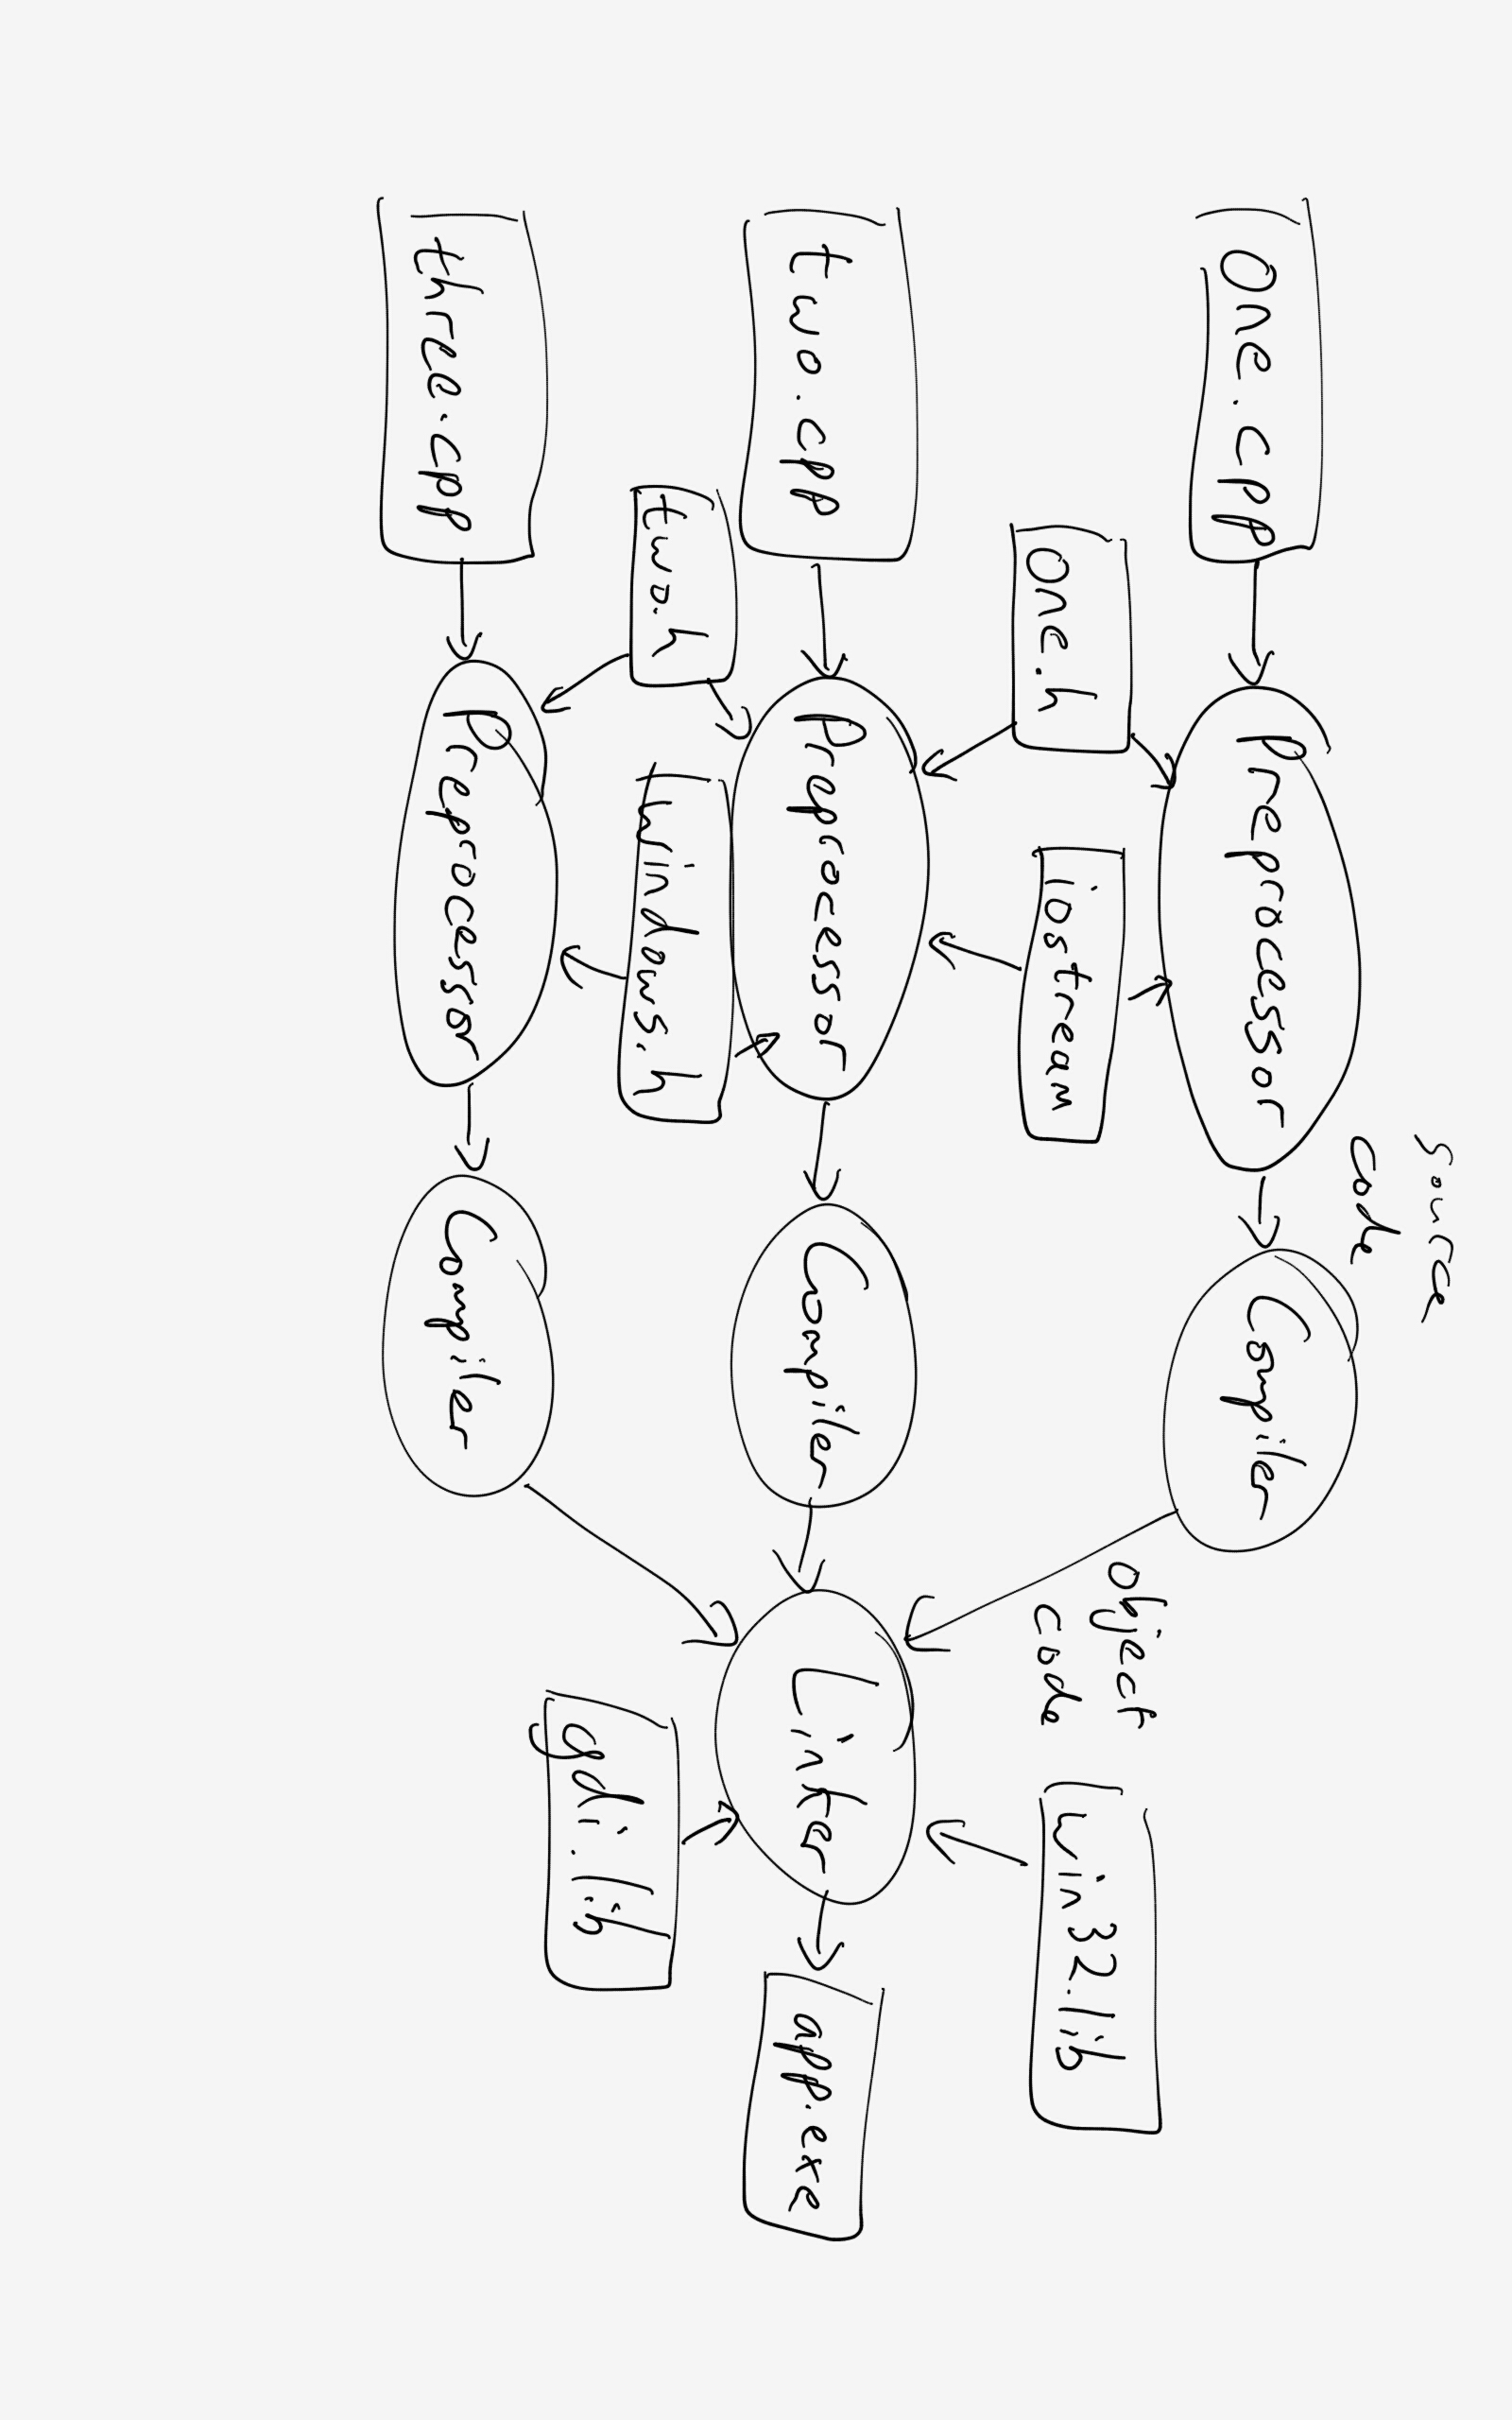
\includegraphics[height=\textwidth,angle=90]{compiler_sketch}
%\end{frame}

\end{document}
